\section{Variedades suaves}

\begin{defi}
Um subconjunto $M \subset \mathbb{R}^3$ é chamado de \emph{superfície regular} se para qualquer $p \in M$ existe um aberto $V$ de $\mathbb{R}^3$ e uma aplicação $\varphi: U \rightarrow M \cap V$ chamada de \emph{parametrização}, onde $U$ e um aberto de $\mathbb{R}^2$, tal que
\begin{enumerate}
    \item $\varphi$ é um homeomorfismo
    \item $\varphi$ é diferenciável e sua diferencial $d\varphi(x): \mathbb{R}^2 \rightarrow \mathbb{R}^3$ é injetora para todo $x \in U$
\end{enumerate}
\end{defi}

\begin{figure}
	\centering
	
	\begin{tikzpicture}
	\draw (0,0) .. controls (3/4,9/4) .. (3,3);
	\draw (3,0) .. controls (4,9/4) .. (7,3);
	\draw (0,0) .. controls (1.5,0.5) .. (3,0);
	\draw (3,3) .. controls (5,3.5) .. (7,3);
	
	\draw (2.5,1.5) ellipse (20pt and 10pt);
	
	\draw[->] (0,-5) -- (7,-5);
	\draw[->] (1,-6) -- (1,-1);
	
	\draw (4,-3) ellipse (50pt and 30pt);
	
	\draw[<-] (3,1.5) parabola (4,-2);
	
	\fill (2.5,1.5) circle (1pt);
	
	\draw (2.5,2.5) node [anchor=north] {$M \cap V$};
	\draw (5,-1.5) node [anchor=north] {$U$};
	\draw (4.5,0) node [anchor=east] {$\varphi$};
	\draw (0,-1) node [anchor=west] {$\mathbb{R}^2$};
	\draw (2.5,1.5) node [anchor=east] {$p$};
	\draw (7,3) node [anchor=west] {$M$};
	\end{tikzpicture}
	\caption{Parametrização de uma superfície}
\end{figure}

\begin{obse}
	Quando $M \cap V = M$, $\varphi$ se chama de \emph{parametrização global}.
\end{obse}

\begin{exemplo}
Seja $f: U \subset \mathbb{R}^2 \rightarrow \mathbb{R}$ uma função diferenciável. Denote por $M$ seu gráfico
\begin{equation*}
    M = \text{Graf}(f) = \{ (x,f(x)): x \in U \}
\end{equation*}

Neste caso $M$ admite uma parametrização global. Defina $\varphi: U \rightarrow M$ pondo
\begin{equation*}
    \varphi(x) = (x,f(x)), x \in U
\end{equation*}
\end{exemplo}

\begin{defi}
Seja $\phi: V \subset \mathbb{R}^m \rightarrow \mathbb{R}^n$ uma aplicação diferenciável. Um ponto $p \in V$ é chamado de \emph{ponto crítico} de $\phi$ se $d\phi(p)$ não é sobrejetora. Um ponto $q \in \mathbb{R}^n$ é chamado de \emph{valor crítico} de $\phi$ se existe algum ponto crítico de $\phi$ em $\phi^{-1}(q)$. Um ponto $q \in \mathbb{R}^n$ que não é valor crítico é chamado \emph{valor regular} para $\phi$.
\end{defi}

\begin{obse}
Quando $n=1$, um ponto $p \in V$ é ponto crítico de $\phi$ se e somente se $d\phi(p)=0$.
\end{obse}

\begin{teo}\label{preimagem_de_um_valor_regular}
Sejam $f: \mathbb{R}^3 \rightarrow \mathbb{R}$ uma função diferenciável e $c \in \mathbb{R}$ um valor regular para $f$. Então, o subconjunto
\begin{equation*}
    M = f^{-1}(c) \text{ é superfície regular.}
\end{equation*}
\end{teo}

\begin{proof}
Seja $p \in M$ tal que $p=(x_0,y_0,z_0)$, então $df(p) \neq 0$. Sem perdida de generalidade podemos dizer que $f_z(p) \neq 0$. Pelo Teorema da Função Implícita \cite[p.~296]{lima1985} \cite[p.~36]{montiel2009}, existem $U$ aberto de $\mathbb{R}^2$ tal que $(x_0,y_0) \in U$, $V$ aberto de $\mathbb{R}$ tal que $z_0 \in V$ e uma função diferenciável $g: U \rightarrow V$ tal que $g(x_0,y_0)=z_0$ e $f(x,y,g(x,y)) = c$ para todo $(x,y) \in U$.

Definamos $\varphi: U \rightarrow U \times V$ tal que $\varphi(x,y) = (x,y,g(x,y))$. Se ve que $\varphi$ é uma parametrização, portanto $M$ é uma superfície.
\end{proof}

\begin{exemplo}
Seja $f: \mathbb{R}^3 \rightarrow \mathbb{R}$ dada por $f(x) = \langle x,x \rangle$. Temos que $f$ é diferenciável e vale
\begin{equation*}
    df(p)v = 2 \langle p,v \rangle
\end{equation*}

para qualquer $p \in \mathbb{R}^3$ e para qualquer $v \in \mathbb{R}^3$. Disso decorre que $0 \in \mathbb{R}^3$ é o único ponto crítico de $f$. Note que
\begin{equation*}
    f(0) = 0 \neq 1.
\end{equation*}

Disso decorre, pelo teorema \ref{preimagem_de_um_valor_regular}, que a esfera $S^2 = f^{-1}(1)$ é uma superfície regular em $\mathbb{R}^3$.
\end{exemplo}

\begin{exemplo}
Seja $S^2 \subset \mathbb{R}^3$ a esfera unitária. Denote por $N$ seu polo norte, $N = (0,0,1)$

\begin{figure}
	\centering
	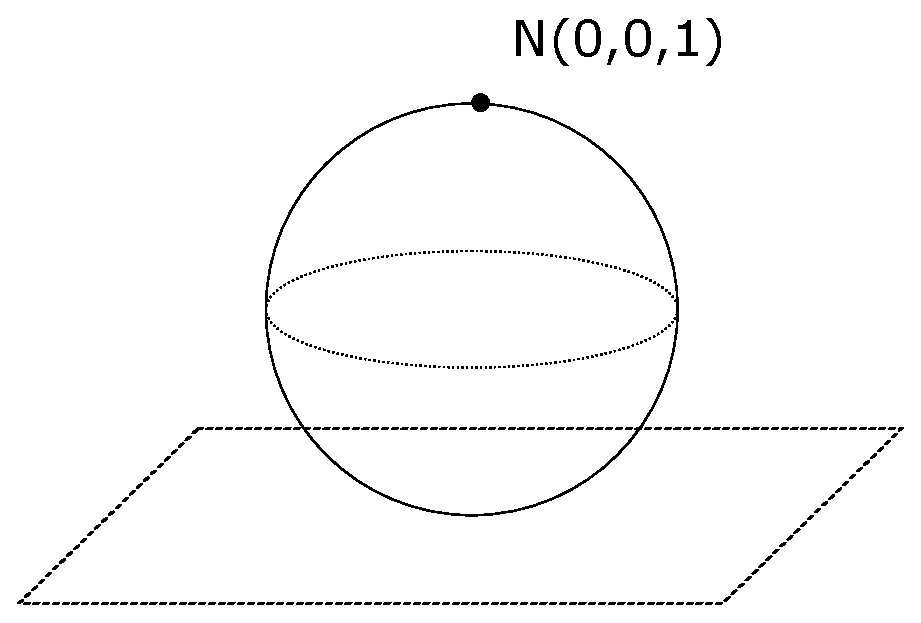
\includegraphics[scale=0.5]{graficos/projecao_estereografica.eps}
\end{figure}

Denote por $\pi_N$ a aplicação que associa a cada ponto $x \in S^2 \setminus \{N\}$ o ponto $\pi_N(x)$ no plano $x_3 = 0$, obtido pela interseção da semirreta que inicia no ponto $N$ e passa pelo ponto $x$ como o plano $x_3 = 0$. Os pontos da semirreta são da forma
\begin{equation*}
    N + t(x - N), t \geq 0.
\end{equation*}

Assim, a semirreta intercepta o plano $x_3 = 0$ quando
\begin{equation*}
    1 + t(x_3 - 1) = 0,
\end{equation*}

ou seja
\begin{equation*}
    t = \frac{1}{1 - x_3}
\end{equation*}

onde $x = (x_1, x_2, x_3)$. Por tanto
\begin{equation*}
    \pi_N(x) = \frac{1}{1-x_3} (x_1, x_2, 0)
\end{equation*}

Portanto $\pi_N$ é diferenciável. Por outro lado, a aplicação $\varphi: \mathbb{R}^2 \rightarrow S^2 \setminus \{N\}$ dada por
\begin{equation*}
	\varphi(x) = \left( \frac{2x_1}{\|x\|^2 + 1}, \frac{2x_2}{\|x\|^2 +1}, \frac{\|x\|^2 -1}{\|x\|^2 +1} \right)
\end{equation*} 

é diferenciável e vale $\pi_N \circ \varphi = \text{Id}$, ou seja, $\pi_N$ é um difeomorfismo.

Analogamente, podemos considerar $\pi_S$, onde $S=(0,0,-1)$.
\end{exemplo}

\begin{defi}
	Seja $M$ um conjunto. Uma \emph{carta local} em $M$ é uma bijeção $\varphi: U \rightarrow \varphi(U)$, onde $U$ é um subconjunto de $M$ e $\varphi(U)$ é um aberto de algum espaço euclideano $\mathbb{R}^n$.
\end{defi}

\begin{defi}
	Duas cartas locais em $M$, $(U, \varphi)$ e $(V, \psi)$, são \emph{compatíveis} se $U \cap V = \emptyset$ ou, se $U \cap V \neq \emptyset$, então $\varphi(U \cap V)$ e $\psi(U \cap V)$ sao abertos de $\mathbb{R}^n$ e a aplicação de transição $\psi \circ \varphi^{-1}$ é um difeomorfismo $C^{\infty}$.
\end{defi}

\begin{defi}
	Um \emph{atlas} $\mathcal{A}$ de dimensão $n$ em $M$ é um conjunto de cartas locais em $M$
	\begin{equation*}
		\mathcal{A} = \{ (U_{\alpha}, \varphi_{\alpha}):  \alpha \in I \}
	\end{equation*}
	
	onde cada $\varphi_{\alpha}(U_{\alpha})$ é aberto em $\mathbb{R}^n$ e $I$ é um conjunto de índices, duas a duas compatíveis e
	\begin{equation*}
		M = \bigcup_{\alpha \in I} U_{\alpha}
	\end{equation*}
\end{defi}

\begin{exemplo}
	Um atlas no espaco euclideano $\mathbb{R}^n$ é dado por
	\begin{equation*}
		\mathcal{A} = \{ (\mathbb{R}^n, \text{Id}) \}
	\end{equation*}
\end{exemplo}

\begin{exemplo}
	Na esfera $S^2$, um atlas é o conjunto
	\begin{equation*}
		\mathcal{A} = \{ (S^2 \setminus \{N\}, \pi_N), (S^2 \setminus \{S\}, \pi_S) \}
	\end{equation*}
	
	onde $\pi_N, \pi_S$ denotam as projeções estereográficas de $S^2$ relativas aos polos norte e sul respectivamente.
\end{exemplo}

\begin{defi}
	Uma carta local $\varphi$ em $M$ é dita \emph{compativel} com um atlas $\mathcal{A}$ em $M$ se $\varphi$ for compativel com todos os elementos do atlas $\mathcal{A}$.
\end{defi}

\begin{lema}
	Seja $\mathcal{A}$ um atlas em $M$. Se $(U, \varphi)$ e $(V, \psi)$ sao duas cartas locais em $M$, ambas compatíveis com $\mathcal{A}$, então $\varphi$ e $\psi$ são compatíveis.
\end{lema}

\begin{defi}
	Um atlas $\mathcal{A}$ em $M$ é dito \emph{maximal} se nao está propriamente contido em nenhum atlas de $M$.
\end{defi}

\begin{lema}
	Dado um atlas $\mathcal{A}$ em $M$, existe um único atlas maximal $\mathcal{A}_{\text{max}}$ em $M$, com $\mathcal{A} \subset \mathcal{A_{\text{max}}}$.
\end{lema}

\begin{lema}
	Dado um atlas $\mathcal{A} = \{ (U_{\alpha}, \varphi_{\alpha}): \alpha \in I \}$ em $M$, existe uma única topologia $\tau_{\mathcal{A}}$ em $M$ que torna cada $U_{\alpha}$ aberto em $M$ e cada carta $\varphi_{\alpha}$ um homeomorfismo, i.e., $\tau_{\mathcal{A}}$ é a \emph{topologia induzida pelo atlas $\mathcal{A}$}.
\end{lema}

\begin{defi}
	Uma \emph{variedade suave} de dimensão $n$ é um par $(M, \mathcal{A})$, onde $M$ é um conjunto e $\mathcal{A}$ é um atlas maximal de dimensão $n$ e classe $C^{\infty}$ em $M$ tal que a topologia induzida $\tau_{\mathcal{A}}$ seja de Hausdorff e satisfaça o segundo axioma da enumerabilidades.
\end{defi}

Gráfico

Sejam $M^2$ uma superfície, $p \in M^2$ e $(U, \varphi)$ carta local em $M^2$, $p \in U$. Como $\varphi(U)$ é aberto de $\mathbb{R}^2$, podemos expressar $\varphi$ como
\begin{equation*}
	\phi(p) = (x(p), y(p)), \forall p \in U
\end{equation*}

As funções $x(p), y(p$ são chamadas \emph{funções coordenadas} de $\varphi$ em $\mathbb{R}^2$.

\begin{nota}
	Para dizer que $\varphi$ está definido pelas funcoes coordenas $x$ e $y$ vamos escrever $\varphi \sim  (x,y)$.
\end{nota}

\begin{defi}
	O \emph{plano tangente} a $M$ num ponto $p \in M$ é o espaço vetorial real (abstrato) de dimensão 2 cuja base natural é
	\begin{equation*}
		\left\{ \frac{\partial}{\partial x} (p), \frac{\partial}{\partial y} (p) \right\}
	\end{equation*}
	
	onde $\frac{\partial}{\partial x}, \frac{\partial}{\partial y}$ são derivadas parciais de $\varphi$ em relação às coordenadas usuais de $\mathbb{R}^2$, i.e.
	\begin{align*}
		\frac{\partial}{\partial x} (p) = d \varphi^{-1} ( \varphi(p) ) e_1\\
		\frac{\partial}{\partial y} (p) = d \varphi^{-1} ( \varphi(p) ) e_2
	\end{align*}
	
	onde $\{ e_1,e_2 \}$ é a base canônica de $\mathbb{R}^2$. Além disso, identificando os vetoes $\frac{\partial}{\partial x} (p), \frac{\partial}{\partial y} (p)$ como derivações temos
	\begin{align*}
		\frac{\partial}{\partial x} (p) (f) = \frac{\partial}{\partial x} \left( f \circ \varphi^{-1} \right) (\varphi(p))\\
		\frac{\partial}{\partial y} (p) (f) = \frac{\partial}{\partial y} \left( f \circ \varphi^{-1} \right) (\varphi(p))
	\end{align*}
	
	onde $f: M \rightarrow \mathbb{R}$ é uma função diferenciável.
\end{defi}

\begin{obse}
	Denote por $T_p M^*$ o espaço dual a $T_p M$, chamado o espaço cotangente a $M$ em $p$. O conjunto $T_p M^*$ também é um espaço vetorial cuja base é $\{ dx(p), dy(p)  \}$ dual à base $\{ \frac{\partial}{\partial x}(p), \frac{\partial}{\partial y}(p) \}$.
\end{obse}

\begin{lembrete}
	Se $E$ é um espaço vetorial real de dimensão $n$ com base $\{ e_1, e_2, \ldots, e_n \}$ sua base dual $\{ f_1, f_2, \ldots, f_n \} \subset E^*$ satisfaz
	\begin{equation*}
		f_i (e_j) = \delta_{ij}, 1 \leq i,j \leq n
	\end{equation*}
\end{lembrete}

	O conjunto
	\begin{equation*}
		TM = \bigcup_{p \in M} T_p M
	\end{equation*}
	
	dado pela união disjunta dos planos tangentes a $M$, é chamado de \emph{fibrado tangente} a $M$, admite uma estrutura de variedades suave de dimensão 4.